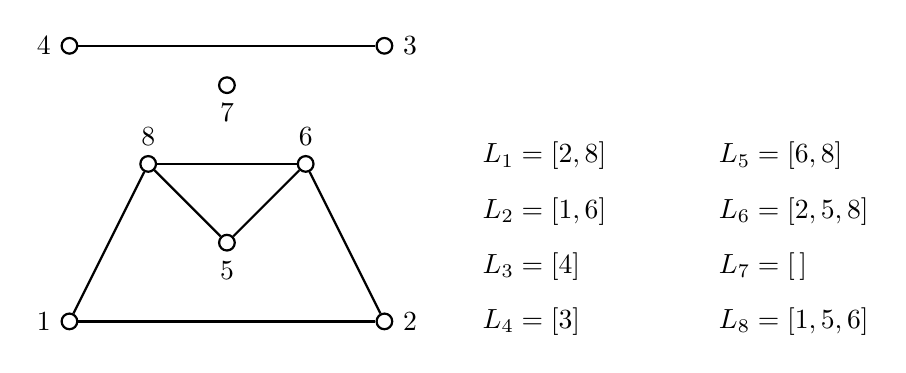
\begin{tikzpicture}
[nodedecorate/.style={shape=circle,inner sep=2pt,draw,thick},%
  linedecorate/.style={-,thick}]
%% nodes or vertices
\foreach \nodename/\x/\y/\direction/\navigate in {
  1/0/0/left/west, 2/4/0/right/east, 3/4/3.5/right/east,
  4/0/3.5/left/west, 5/2/1/below/south, 6/3/2/above/north,
  7/2/3/below/south, 8/1/2/above/north}
{
  \node (\nodename) at (\x,\y) [nodedecorate] {};
  \node [\direction] at (\nodename.\navigate) {$\nodename$};
}
%% adjacency lists
\node (L1) at (5,2.1) [] {};
\node [right] at (L1.east) {$L_1 = [2,8]$};
\node (L2) at (5,1.4) [] {};
\node [right] at (L2.east) {$L_2 = [1,6]$};
\node (L3) at (5,0.7) [] {};
\node [right] at (L3.east) {$L_3 = [4]$};
\node (L4) at (5,0) [] {};
\node [right] at (L4.east) {$L_4 = [3]$};
\node (L5) at (8,2.1) [] {};
\node [right] at (L5.east) {$L_5 = [6,8]$};
\node (L6) at (8,1.4) [] {};
\node [right] at (L6.east) {$L_6 = [2,5,8]$};
\node (L7) at (8,0.7) [] {};
\node [right] at (L7.east) {$L_7 = [\,]$};
\node (L8) at (8,0) [] {};
\node [right] at (L8.east) {$L_8 = [1,5,6]$};
%% edges or lines
\path
\foreach \startnode/\endnode in {1/2, 1/8, 2/6, 3/4, 5/6, 5/8, 6/8} {
  (\startnode) edge[linedecorate] node {} (\endnode)
};
\end{tikzpicture}
